\documentclass{article}

\usepackage{natbib}

\usepackage[utf8]{inputenc} % allow utf-8 input
\usepackage[T1]{fontenc}    % use 8-bit T1 fonts
\usepackage{hyperref}       % hyperlinks
\usepackage{url}            % simple URL typesetting
\usepackage{booktabs}       % professional-quality tables
\usepackage{amsfonts}       % blackboard math symbols
\usepackage{nicefrac}       % compact symbols for 1/2, etc.
\usepackage{microtype}      % microtypography

\usepackage{amsthm,amsmath,amssymb}
\usepackage{macros}
\usepackage{subcaption}
\usepackage[textfont=small, labelfont=small]{caption}
\usepackage{graphicx}
\DeclareGraphicsExtensions{.pdf,.png,.jpg,.eps}

\usepackage{algorithm}
\usepackage{algorithmic}

\usepackage[color=yellow]{todonotes}
\usepackage{booktabs}
\usepackage[inline]{enumitem}
\usepackage{verbatim}

\usepackage[left=1.5in, right=1.5in, top=1.25in, bottom=1.25in]{geometry}

\usepackage{setspace}


\title{Discrete and continuous latent states of neural activity in \textit{Caenorhabditis Elegans}}

\author{Scott W. Linderman,
  David M. Blei,
  and
  Liam Paninski \\
  Columbia University
}

\begin{document}

\singlespacing
\maketitle

\begin{abstract}
  Recent advances in neural recording technologies have enabled
  simultaneous measurements of the majority of head ganglia neurons in
  immobilized \celegans~\citep{kato2015global}. Moreover, since some
  neurons are known to reliably indicate the onset or offset of
  particular behaviors, like ventral and dorsal turns, behavioral
  state can be decoded from the simultaneous population recordings.
  These datasets provide unique visibility into the relationship
  between neural activity and behavior.  While it seems clear that
  activity is inherently lower dimensional than the number of neurons
  due to strong correlations between cells, the nature of the latent brain state
  remains unclear. For example, is brain state better thought of as
  discrete or continuous, or perhaps a combination of the two? Does it
  obey linear or nonlinear dynamics?  We propose a generative approach
  to probing these questions. We model the neural activity as a
  \emph{switching linear dynamical system} (SLDS), with both discrete
  and continuous latent states, and conditionally linear dynamics.  We
  then analyze the posterior distribution over states implied by the
  neural recordings and find that the discrete states correspond to
  stereotypical motor sequences. In contrast to previous work, these
  states are exposed in an entirely unsupervised manner.
\end{abstract}

% Body
\onehalfspacing

\section{Introduction}
% The world as it was:
The nematode \celegans~is unique among the model organism of
neuroscience. For decades, we have known the connectome of its 302
neurons, yet a comprehensive understanding of hows its neural activity
reflects sensory processes and produces behavior still eludes
us. While this connectome, or wiring diagram, has provided invaluable
information about the structure of these neural circuits, the critical
missing piece has been large scale functional measurements of these
circuits in action. With the advent of optical recording technologies,
we now possess a mounting set of tools for measuring the activity of large
fractions of these neurons simultaneously. These technologies provide
exciting opportunities to probe the link between neural activity,
sensory processing, and, ultimately, behavior.

Recently, \citet{kato2015global} have harnessed these methodological
advances to study the coordinated activity of hundreds of neurons
in head-fixed \celegans. Across multiple organisms, they have found that
neural activity reliably traces out smooth trajectories in the subspace
spanned by the first three principal components.
% TODO: Figure showing these trajectories
Upon closer evaluation, they have found that different components of these
trajectories correspond to different elements of behavior, like
forward and reverse crawling, dorsal and ventral turns, etc. These
results raise a number of interesting questions: can we learn a
(potentially nonlinear) dynamical system that approximates these
low-dimensional dynamics; is there a more appropriate subspace, or
collection of subspaces, for capturing these dynamics; can we gain
statistical power by partial, noisy recordings across separate worms
and trials; and, can we segment these trajectories in an unsupervised
manner to glean further insight into the relationship between
low-dimensional state and behavior?

% Then one day:
We have developed a probabilistic framework for investigating these questions.
The findings of \citet{kato2015global} --- namely, that neural activity
is low dimensional with behavior-specific dynamics --- suggest that
these multineuronal recordings may be aptly modeled in terms of
a dynamic, low-dimensional latent states. Moreover, they suggest
that neural activity may be parsed into a sequence of discrete
actions, like turning or crawling forward. These two properties are
naturally combined by \emph{switching linear dynamical systems} (SLDS),
a class of probabilistic time series characterized by co-evolving
discrete and continuous latent states.  We have extended this
class of models with a hierarchical Bayesian framework that captures
many of the nuances of these whole-brain recordings. In fitting these
models to recordings from multiple \celegans, we characterize the
globally nonlinear dynamics that govern neural activity, and we
parse these recordings into an interpretable sequence of behavioral segments.

% Raising the stakes:
% Moment of truth:
% World as it is now:
The remainder of this paper is structured as follows. In Section~\ref{sec:slds}
we introduce the class of swithing linear dynamical systems and provide
some insight into the latent states and model parameters. Section~\ref{sec:hslds}
develops a hierarchical extension of the SLDS to share statistical
strength by combining recordings from multiple organisms with partially
overlapping sets of observed neurons.  Then, Section~\ref{sec:results}
presents results of applying these models to a set of recordings from
five separate \celegans. We conclude with directions for further research.


\section{Switching Linear Dynamical Systems}
\label{sec:slds}

\begin{figure}[t]
\centering%
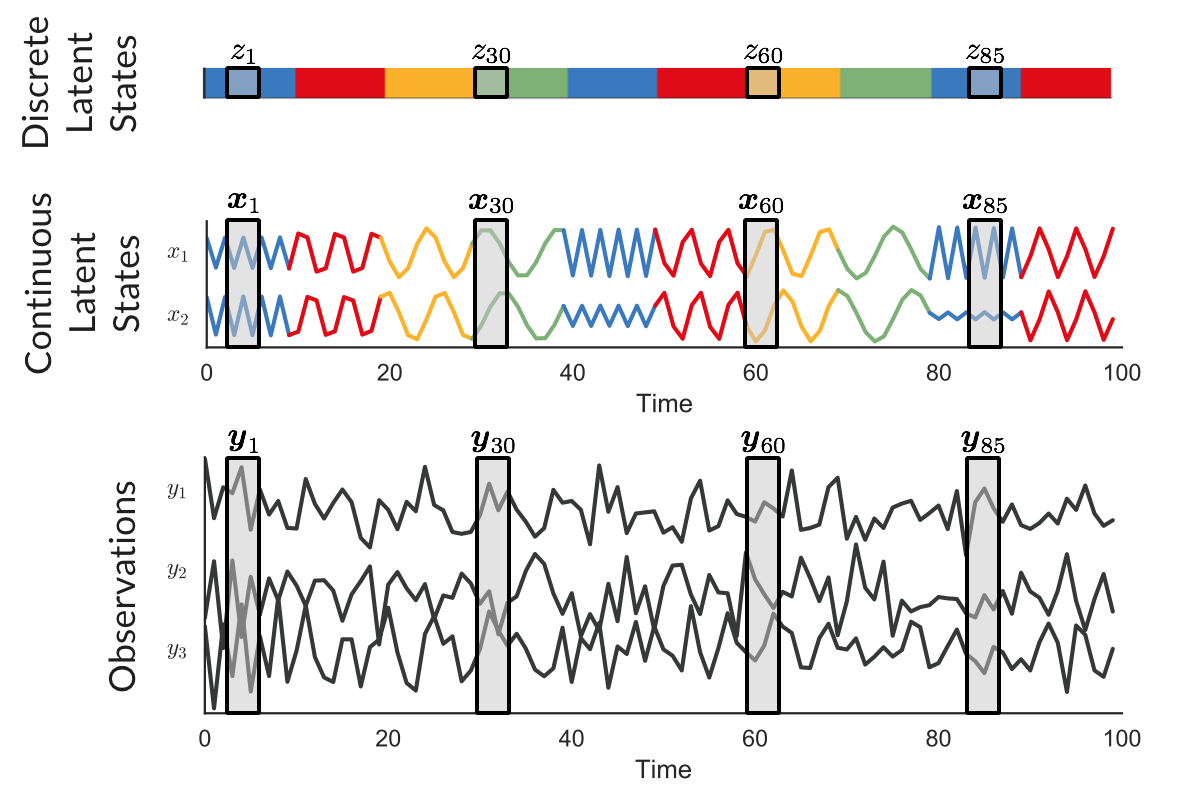
\includegraphics[width=5.5in]{slds.png} 
\caption{Simulated data from a switching linear dynamical system.  The
  population stochastically switches between discrete states,~$z_t \in
  \{1,\ldots,K\}$ (here,~$K=4$), each of which is color coded for
  visualization.  These discrete states govern the linear dynamics of
  the continuous latent state,~$\bx_t \in \reals^D$ (here,~$D=2$). For
  example, these states correspond to oscillatory dynamics with
  different frequencies. Finally, the observed signals,~$\by_t \in
  \reals^N$ (here,~$N=8$), are obtained via a linear transformation of
  the underlying, continuous state,~$\bx_t$, plus Gaussian noise. The
  correlations and dynamics in the observations are inherited from the
  dynamics of the latent states.}
\label{fig:slds_ex}
\end{figure}

Assume the instantaneous neural activity at time~$t$ for a population
of~$N$ neurons is represented as a vector,~$\by_t \in \reals^N$. In
calcium imaging settings, the entries in this vector may be
instaneous~$\Delta F/F$ measurements, or another signal that captures
neural activity. In this experiment, we use the smoothed time
derivative of~$\Delta F/F$. Over the course of an experiment, we
measure a sequence of vectors, which we combine into a matrix denoted
by~$\by_{1:T}$.

The SLDS model is based on the following assumptions: (i) the instantaneous
neural activity,~$\by_t$, reflects an underlying, low-dimensional
latent state; (ii) this state has a discrete component,~$z_t \in \{1, \ldots, K\}$,
and a continuous component,~$\bx_t \in \reals^D$; (iii) the continuous
latent state has linear dynamics governed by the corresponding discrete
latent state; and (iv) the observed neural activity is a linear function
of the underlying states with additive Gaussian noise.  Assumptions (i)
and (iv) are justified by the low-dimensional trajectories that
\citet{kato2015global} revealed with PCA (a linear dimensionality
reduction method). Assumptions (ii) and (iii) follow from the
trajectories naturally segment into discrete units, each with relatively
simple dynamics. 

These assumptions are formalized with the following generative model:
\begin{align}
  \label{eq:joint}
  p(\by_{1:T}, \bx_{1:T}, \bz_{1:T} \given \bTheta) &= 
  p(\bTheta)
  \prod_{t=1}^T
  p(z_t \given z_{t-1}, \bTheta) \, 
  p(\bx_t \given z_{t-1}, \bx_{t-1}, \bTheta) \, 
  p(\by_t \given z_t, \bx_t, \bTheta).
\end{align}
Beliefs about the dynamics of these latent states are encoded in the 
form of the conditional distributions for~$z_t$ and~$\bx_t$. First,
we assume the discrete states follow a Markov process,
\begin{align}
  p(z_t \given z_{t-1}, \bTheta) &\sim \bpi^{(z_{t-1})}.
\end{align}
Next, the continuous latent state is imbued with linear Gaussian dynamics,
\begin{align}
  p(\bx_t \given \bx_{t-1}, z_{t-1}, \bTheta) 
  &\sim \distNormal(\bA^{(z_{t-1})} \bx_{t-1} + \bb^{(z_{t-1})}, \bQ^{(z_{t-1})}).
\end{align}

% Figure illustrating latent dynamics
\begin{figure}[t]
\centering%
\begin{subfigure}{.24\textwidth}
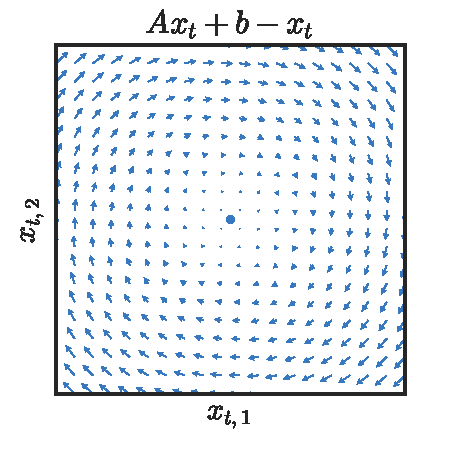
\includegraphics[width=\textwidth]{rotation_1}
\end{subfigure} 
\begin{subfigure}{.24\textwidth}
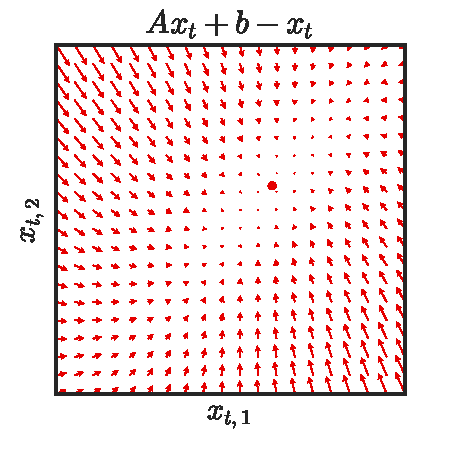
\includegraphics[width=\textwidth]{rotation_2}
\end{subfigure} 
\begin{subfigure}{.24\textwidth}
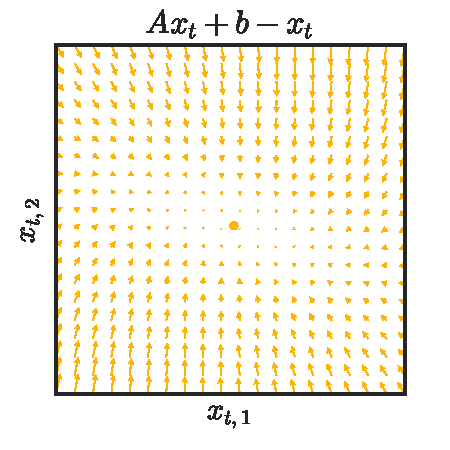
\includegraphics[width=\textwidth]{rotation_3}
\end{subfigure} 
\begin{subfigure}{.24\textwidth}
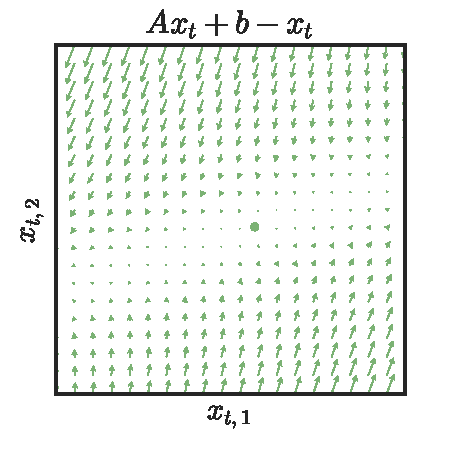
\includegraphics[width=\textwidth]{rotation_4}
\end{subfigure} 
\caption{The dynamics corresponding to discrete latent state~$k$ may
  be visualized as a vector field where the arrows point to the
  expected next state,~$\bbE[\bx_{t+1}]=\bA^{(k)}\bx_t + \bb^{(k)}$.
Here, we show the dynamics for the first and fourth discrete states 
in the synthetic example from Figure~\ref{fig:slds_ex}. The first 
discrete state is a random walk with a slight decay toward the origin;
the fourth discrete state corresponds to fast, oscillatory dynamics.}
\label{fig:slds_dynamics_ex}
\end{figure}


Finally, we impose the assumption of linear observations via the conditional
distribution,
\begin{align}
  p(\by_t \given \bx_{t}, z_{t}, \bTheta) 
  &\sim \distNormal(\bC^{(z_{t})} \bx_{t} + \bd^{(z_{t})}, \bR^{(z_t)}).
\end{align}
Thus, the parameters of the model are,
\begin{align}
  \bTheta &= \left\{ \bA^{(k)}, \bb^{(k)}, \bQ^{(k)}, \bC^{(k)}, \bd^{(k)}, \bR^{(k)}, \bpi^{(k)} \right\}_{k=1}^K .
\end{align}

Figure~\ref{fig:slds_ex} illustrates a sample from this generative model.
The observations are a sequence of vectors, in this case they are ~$N=3$ dimensional
vectors,~$\by_t$.  These states are a noisy, linear projection of an underlying
continuous latent state,~$\bx_t$, which is~$D=2$ dimensional in this case.
Here, the continuous state switches between~$K=4$ discrete regimes (four
different colors), each corresponding to different frequencies of oscillation.
The discrete state, encoded by~$z_t \in \{1, 2, 3, 4\}$ (blue, red, yellow, green),
follows a simple Markov process with transition matrix~${\bP = \{\pi^{(k)}\}_{k=1}^K}$
(not shown).

How should we interpret the these parameters? Linear dynamical
systems can essentially capture simple dynamics, like rotations, exponential
growth, and exponential decay. The stability of the system is determined
by the eigenvalues of the dynamics matrix,~$\bA^{(k)}$ --- if the eigenvalues
all have modulus less than one, the system is asymptotically stable, and
converges to a fixed point at~$(\bI - \bA^{(k)})^{-1} \bb^{(k)}$. If
the largest eigenvalue is exactly one, the system oscillates in perpetuity.
If any eigenvalue exceeds one in magnitude, the system diverges exponentially
quickly.  A variety of linear dynamical systems are illustrated in
Figure~\ref{fig:slds_dynamics_ex}. All of these systems are stable, and their
fixed points are shown as dots.

% Nonlinearity of compositional system
While the capacity of linear dynamical systems is somewhat limited,
the composition of many linear dynamical modes, as in an SLDS, yields
a highly nonlinear system. This is particularly important for modeling
neural data, which is believed to have nonlinear and often behavior-dependent
dynamics.

Given observations,~$\by_{1:T}$, our goal is to infer the discrete
latent states,~$bz_{1:T}$, and the continuous latent states,~$\bx_{1:T}$,
as well as to learn the parameters,~$\bTheta$.  We take a Bayesian
approach, specifying conjugate prior distributions for the parameters,
and using Markov chain Monte Carlo (MCMC) to estimate the posterior
distribution of the parameters and states given the observed data.
Details of this MCMC algorithm are provided in Appendix~\ref{app:mcmc}.



\section{Hierarchical Switching Linear Dynamical Systems}
\label{sec:hslds}

\begin{figure}[t]
\centering%
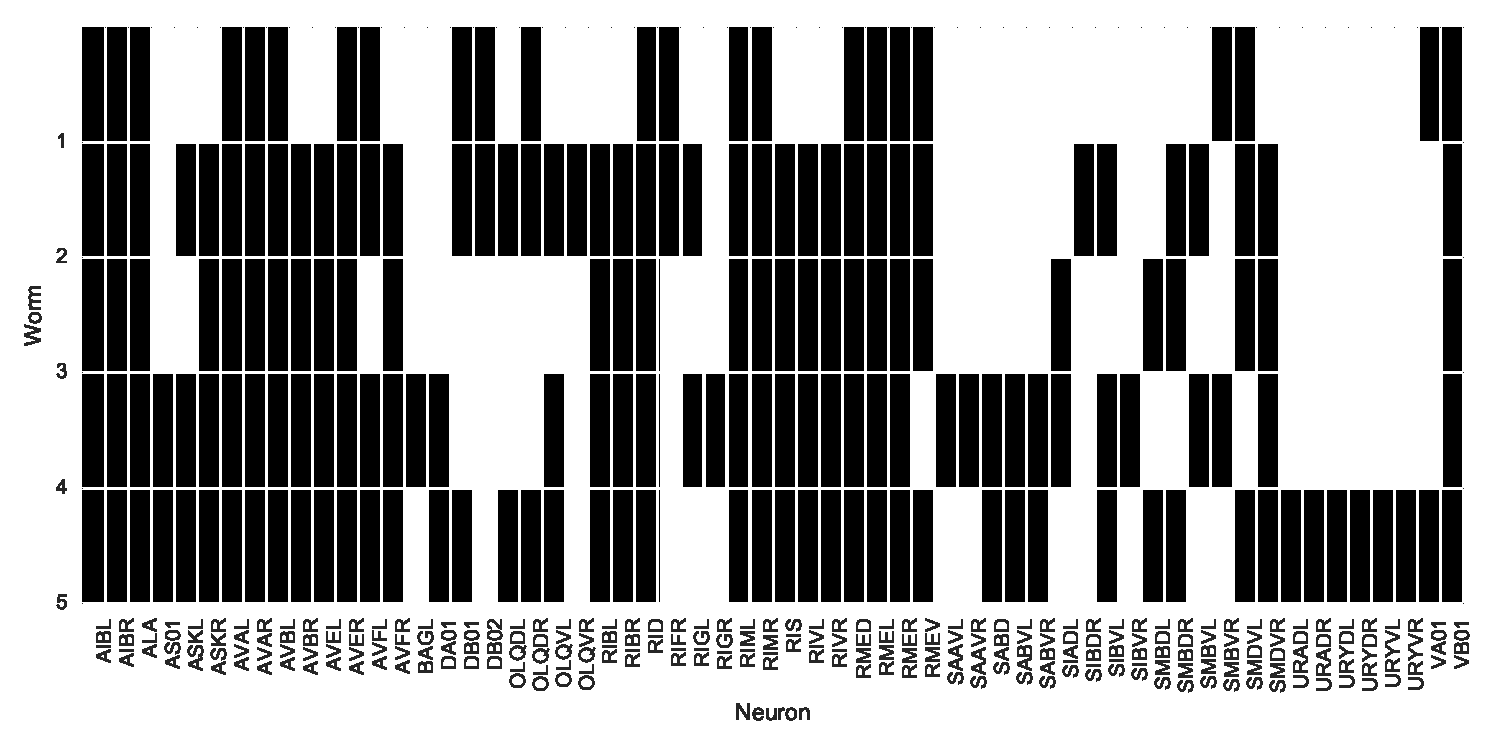
\includegraphics[width=5.5in]{identified_neurons.pdf} 
\caption{Identified neurons in the five worms from \citet{kato2015global}.
  Across all five worms, these 60 labeled neurons were identified in at
  least one worm. In addition to these labeled neurons,
  each worm contains roughly 70 unlabeled neurons that inform our
  estimate of that worm's latent states, but which we cannot share
  across worms. }
\label{fig:identified_neurons}
\end{figure}


The neural recordings of \citet{kato2015global} present additional
opportunities to extend the SLDS. In these experiments, recordings
have been made in five separate worms. Each recording contains roughly
100 of the worm's 302 neurons, but the subset of observed neurons
varies from worm to worm. Moreover, while each of these 302 neurons
has a unique name, only about 30 out of the 100 neurons could be
reliably identified in each recording. For example, in the recording
of worm A, we may observe 100 neurons of which 30 have been identified
as, say, {AAV}, {RIM}, etc., while the remaining 70 are unidentified.
Figure~\ref{fig:identified_neurons} shows the 60 labeled neurons which
were identified in at least one of the worms. For example, ABL is
identified in all five worms, whereas SIADL is only found in the
second worm.  In addition to these identified neurons, we also have
roughly 70 unlabeled neurons for each worm. While these unlabeled
neurons do not provide information that can be shared across worms,
they do provide information about that worm's latent states.  Our goal
is to combine these recordings to extract a shared model of the neural
dynamics of \celegans.

\begin{figure}[t]
\centering%
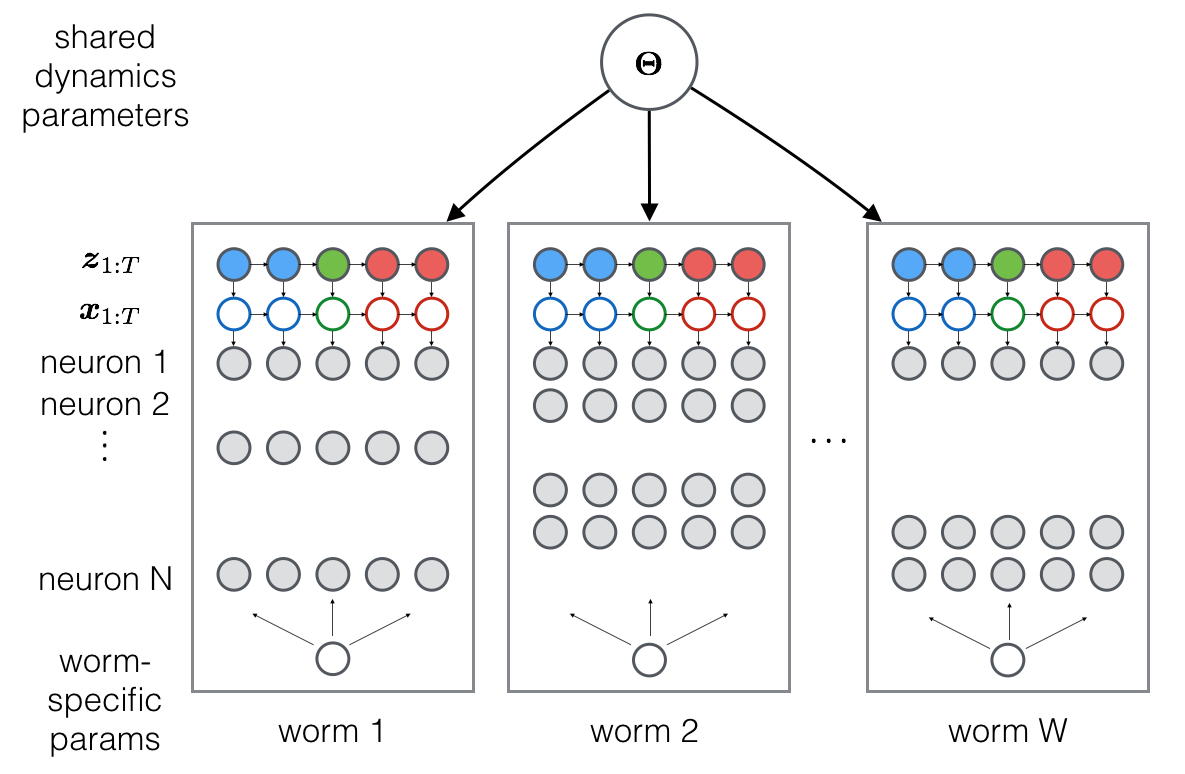
\includegraphics[width=5.5in]{hslds.png} 
\caption{A schematic of the hierarchical SLDS for combining information
  across multiple worms in order to learn a shared dynamical system
  for \celegans.  We have a set of shared set of model parameters,~$\bTheta$,
  represented by the large node at the top of the graphical model. Each
  worm,~$w$ has its own set of discrete latent states (colored nodes)
  and continuous latent states (nodes with colored outlines) and observed neurons.
  For example, neuron 1 may appear in all neurons whereas neuron 2
  may only be seen in worm 2. Thus, each worm provides information
  about the mapping from latent states to observations for only a
  subset of neurons. In terms of the model, this corresponds to a
  subset of rows in the matrix~$\bC$ and the vector~$\bd$. Finally,
  we allow each worm to have local parameters that capture, for example,
  the amount of fluorescent protein expressed in a particular neuron
  for a given worm. 
}
\label{fig:hslds}
\end{figure}

We propose the following hierarchical SLDS (hSLDS) to combine data from
multiple worms. Since these worms are genetically identical, we hypothesize
that their dynamics should be the same. That is, they share the same set
of~$K$ discrete states, as well as the
parameters~$\{\bA^{(k)}, \bb^{(k)}, \bQ^{(k)}, \bpi^{(k)}\}_{k=1}^K$.
We assume the following mapping from latent states to the neural activity
of worm~$w$, time~$t$, and neuron~$n$:
\begin{align}
  y_{w,t,n} &= \gamma_{w,n} \bc_n^\trans \bx_{w,t} + d_{w,n} + \epsilon_{w,t,n}, \\
  \epsilon_{w,t,n} &\sim \distNormal(0, r_{w,n}^2).
\end{align}
Thus, the mapping from latent states to the activity of neuron~$n$ is
partially shared across worms, in that all worms share the
vector~$\bc_n$.  These constitute the rows of an emission
matrix,~$\bC$. Note that, for simplicity, we have required all
discrete states,~$z_t$ to share the same emission matrix. However, we
have introduced a set of worm-specific parameters,~$\{\gamma_{w,n},
d_{w,n}, r_{w,n}\}$. The gain,~$\gamma_{w,n}$, captures differences in
amplitude of the neural signal that may arise from variation in
fluorescent protein expression from worm to worm.  Likewise, the
bias,~$d_{w,n}$, accounts for different baseline levels of
activity. Finally, the noise variance,~$r_{w,n}^2$, enables neuron~$n$
to have different marginal variance from worm to worm, which may arise
due to a number of factors, like protein expression levels and the
clarity of a particular recording.  Figure~\ref{fig:hslds} provides a
graphical representation of this model.

\section{Results}
\label{sec:results}

\bibliographystyle{plainnat}
\bibliography{writeup}

\appendix

\section{Bayesian Inference for Switching Linear Dynamical Systems}
\label{app:mcmc}
Our goal is to estimate the posterior probability of a sequence 
of latent states and a set of parameters given the observed data.
From Bayes' rule, we have,
\begin{align}
  p(\bz_{1:T}, \bx_{1:T}, \bTheta \given \by_{1:T}) 
  &= 
  \frac{p(\by_{1:T}, \bx_{1:T}, \bz_{1:T}, \bTheta)}{p(\by_{1:T})}.
\end{align}
The numerator is the joint probability given by Eq.~\eqref{eq:joint}, and
the denominator,~$p(\by_{1:T})$, which is also known as the
\emph{marginal likelihood}, is given by an integral over possible
latent states and parameters,
\begin{align}
  p(\by_{1:T}) &= \int p(\by_{1:T}, \bx_{1:T}, \bz_{1:T}, \bTheta) 
  \, \mathrm{d}\bx_{1:T} \, \mathrm{d}\bz_{1:T} \, \mathrm{d}\bTheta.
\end{align}
Unfortunately, this integral is not efficiently computable for complex
models like the SLDS, forcing us to seek approximate inference methods
instead. Markov chain Monte Carlo (MCMC) methods \todo{cite} offer one
such approach. 

To construct our MCMC algorithm, we iteratively sample one set of 
latent states or parameters from its conditional distribution, holding 
the rest fixed, in a technique known as Gibbs sampling \todo{cite}. 
There are five main sets of parameters to sample, detailed below.
\begin{enumerate}
  \item \textit{Gibbs sampling the discrete latent states,~$\bz_{1:T}$:}
    
    Given the continuous latent states,~$\bx_{1:T}$, and the
    parameters,~$\bTheta$, the conditional distribution over discrete
    latent states is the same as in a standard hidden Markov model. A
    joint sample from~$p(\bz_{1:T} \given \bx_{1:T}, \by_{1:T},
    \bTheta)$ can be generated using the forward filtering backward
    sampling (FFBS) algorithm.

  \item \textit{Gibbs sampling the continuous latent states,~$\bx_{1:T}$:}
    
    Given the discrete latent states,~$\bz_{1:T}$, the observations,~$\by_{1:T}$,
    and the parameters,~$\bTheta$, the conditional distribution of the 
    continuous latent states is linear and Gaussian. As with the discrete
    latent states, a joint sample of~$p(\bx_{1:T} \given \bz_{1:T}, \by_{1:T}, \bTheta)$
    can be generated using an FFBS algorithm.

  \item \textit{Gibbs sampling the dynamics parameters,~$\{\bA^{(k)}, \bb^{(k)}, \bQ^{(k)}\}_{k=1}^K$:}
    
    For fixed latent state sequences, the dynamics model reduces to a simple 
    multivariate regression problem. We have,
    \begin{multline}
      p(\bA^{(k)}, \bb^{(k)}, \bQ^{(k)}  \given \bz_{1:T}, \bx_{1:T}, \by_{1:T}, \bTheta)
      \\ 
      \propto
      p(\bA^{(k)}, \bb^{(k)}, \bQ^{(k)})
      \prod_{t=1}^T \left[ \,
        \distNormal(\bx_{t} \given \bA^{(k)} \bx_{t-1} + \bb^{(k)},\, \bQ^{(k)} \right]^{\bbI[z_{t-1}=k]}.
    \end{multline}
    If the prior distribution is the form of a matrix normal inverse Wishart (MNIW) prior, 
    then this conditional distribution will be as well. 

  \item \textit{Gibbs sampling the observation parameters,~$\{\bC^{(k)}, \bd^{(k)}, \bR^{(k)}\}_{k=1}^K$:}
    
    As with the dynamics parameters, 
    for fixed latent state sequences, the observation model is also a 
    multivariate regression problem. We have,
    \begin{multline}
      p(\bC^{(k)}, \bd^{(k)}, \bR^{(k)}  \given \bz_{1:T}, \bx_{1:T}, \by_{1:T}, \bTheta)
      \\ 
      \propto
      p(\bC^{(k)}, \bd^{(k)}, \bR^{(k)})
      \prod_{t=1}^T \left[ \,
        \distNormal(\by_{t} \given \bC^{(k)} \bx_{t} + \bd^{(k)},\, \bR^{(k)} \right]^{\bbI[z_{t}=k]}.
    \end{multline}
    This, too, is conjugate when the prior distribution assumes the
    form of a matrix normal inverse Wishart (MNIW) distribution.

  \item \textit{Gibbs sampling the Markov parameters,~$\{\bpi^{(k)}\}_{k=1}^K$:}
    
    Finally, we must sample the Markov transition matrix. We separate
    this into its~$K$ rows, each of which specifies a probability
    distribution,~$p(z_t \given z_{t-1}=k) = \bpi^{(k)}$.  For a fixed
    discrete latent state sequence, the conditional distribution of~$\bpi^{(k)}$ 
    is,
    \begin{align}
      p(\bpi^{(k)} \given \bz_{1:T}) &\propto
      p(\bpi^{(k)}) \prod_{t=1}^T \left[ \pi_{z_t}^{(k)} \right]^{\bbI[z_{t-1}=k]}.
    \end{align}
    If the prior distribution is~$p(\bpi^{(k)}) = \distDirichlet(\bpi^{(k)} \given \alpha)$, then this
    conditional distribution is a Dirichlet as well,
    \begin{align}
      p(\bpi^{(k)} \given \bz_{1:T}) 
      &= \distDirichlet(\bpi^{(k)} \given \widetilde{\balpha}^{(k)}) \\
      \widetilde{\alpha}_{k'}^{(k)} &= \alpha + \sum_{t=1}^T \bbI[z_t = k'] \, \bbI[z_{t-1}=k].
    \end{align}
\end{enumerate} 

Each one of these five steps leaves the desired posterior distribution as the 
unique stationary distribution of the Markov chain. Thus, by iterating these 
steps, the sampled states and parameters will eventually be distributed according
to their posterior probability given the observed data. Critically, the rate 
at which the Markov chain converges to its stationary distribution is determined
in part by the correlation between the sampled latent states at one iteration and
those at the next. If the chain only makes minor updates to the latent state sequence,
it will likely take a long time to converge to the desired posterior distribution.  
By performing joint, ``block'' updates of~$\bx_{1:T}$ and~$\bz_{1:T}$ in steps 
1 and 2, we find that the latent state sequences are able to be explored more 
efficiently.

\end{document}
